\documentclass[border=10pt]{standalone}
\usepackage{pgfplots}
\pgfplotsset{compat=1.18}
\begin{document}
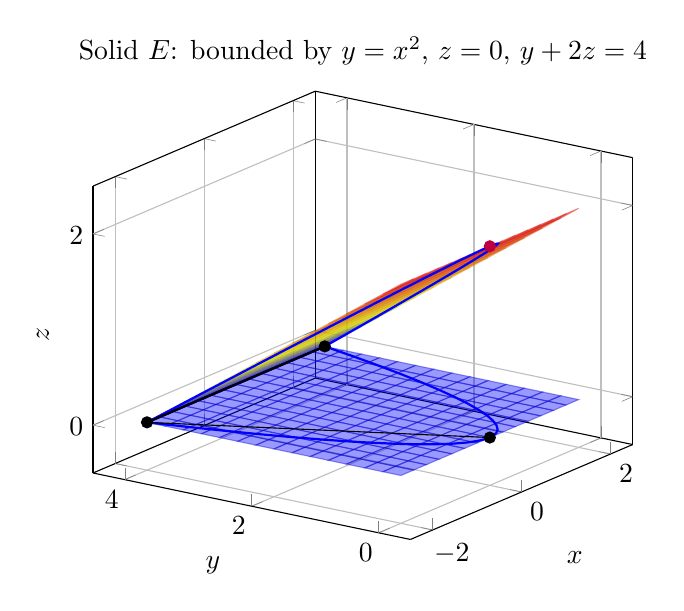
\begin{tikzpicture}
\begin{axis}[
    title={Solid $E$: bounded by $y=x^2$, $z=0$, $y+2z=4$},
    xlabel={$x$}, ylabel={$y$}, zlabel={$z$},
    xmin=-2.5, xmax=2.5, ymin=-0.5, ymax=4.5, zmin=-0.5, zmax=2.5,
    view={-55}{22},
    grid=major,
]
% Bottom face z = 0 (within region y >= x^2)
\addplot3[surf, opacity=0.4, mesh/ordering=y varies, domain=-2:2, domain y=0:4, samples=15, samples y=15] 
    {0};
% Top face z = (4-y)/2
\addplot3[surf, opacity=0.4, mesh/ordering=y varies, domain=-2:2, domain y=0:4, samples=15, samples y=15] 
    {(4-y)/2};
% Edges
\addplot3[domain=-2:2, samples=30, blue, thick] ({x}, {x^2}, {0});
\addplot3[domain=-2:2, samples=30, blue, thick, dashed] ({x}, {x^2}, {(4-x^2)/2});
\addplot3[black, thick] coordinates {(-2,4,0) (2,4,0)};
% Vertex at top of solid (0,0,2)
\addplot3[purple, mark=*, mark size=2pt] coordinates {(0,0,2)};
\addplot3[black, mark=*, mark size=2pt] coordinates {(0,0,0) (-2,4,0) (2,4,0)};
\end{axis}
\end{tikzpicture}
\end{document}